\scanpage{209}

\figure{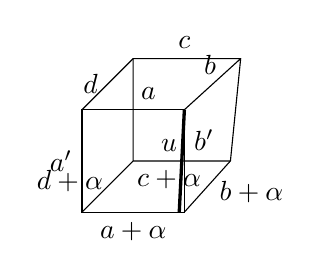
\begin{tikzpicture}[scale=.65]
\draw (0,0)--(0,2)--(2,2)--(2,0)--cycle;
\draw (0,2)--(1,3)--(3.1,3)--(2.9,1)--(2,0) (2,2)--(3.1,3);
\draw (0,0)--(1,1)--(1,3) (1,1)--(2.9,1);
\draw[very thick] (1.9,0)--(2,2);
\node[above] at (1.3,2) {$a$};\node[above] at (2.5,2.5) {$b$};
\node[above] at (2,3) {$c$};\node[left] at (.5,2.5) {$d$};
\node[left] at (0,1) {$a'$};\node[right] at (2,1.4) {$\unsure{b'}$};
\node[below] at (1,0) {$a+\alpha$};\node[right] at (2.5,.4) {$b+\alpha$};
\node[below] at (1.7,1) {$c+\alpha$};\node[left] at (.6,.6) {$d+\alpha$};
\node[above] at (1.7,1) {$\deleted{\unsure{u}}$};
\end{tikzpicture}}

\figure{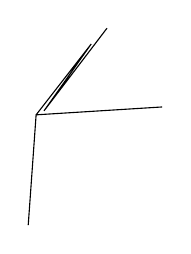
\begin{tikzpicture}
\draw (0,-1.4)--(.1,0)--(1.7,.1);
\draw (.1,0)--(.8,.9)--(.2,.05)--(1,1.1);\end{tikzpicture}}

\figure{\begin{tikzpicture}[scale=1.1]
\draw (0,0)--(0,3);\draw[->] (0,3)--(3.8,3.15);
\draw (3.8,2.95)--(3.65,.1) (0,-.1)--(3.7,-.1);
\draw (0,3.15)--(1.8,4.6) (1.9,4.75)--(5.8,4.95)--(5.45,1.4);
\draw (3.9,3.2)--(5.8,4.95) (3.85,-.1)--(5.5,1.25);
\draw (2,1.25)--(5.3,1.35) (.1,0)--(.9,.55) (1.65,1.5)--(1.65,2.15);
\node[draw,ellipse] at (2.4,3.3) {$a$};\node[draw,ellipse] at (4.55,4) {$b$};
\node[draw,ellipse] at (3.75,5.12) {$c$};\node[draw,ellipse] at (.55,4.05) {$d$};
\node[draw,ellipse] at (-.3,1.2) {$u$};
\node[right] at (3.8,1.55) {$v=u\unsure{-|\cdot}(d-b)$};
\node[right,rotate=12] at (5.65,2.65) {$v+(c-a)=u-(d-b)+(c-a)$};
\node[above] at (1.65,2.3) {$u+c-a$};
\node[above] at (2.7,1.3) {$c+\alpha$};\node[right] at (4.5,.6) {$b+\alpha$};
\node[above] at (.75,.7) {$d+\alpha$};\node[above] at (2.2,-.1) {$a+\alpha\to$};
\node[draw,ellipse] at (2.8,.1) {$\unsure{a'|a''}$};
\end{tikzpicture}}
\[\boxed{d-b=u-v}=d-b\unsure{-=|=}u-v\]
i.e.
\[d+v=b+u\]
\[d-u=b-v\]
\[
a,b,c,d,\underset{\substack{|\\\text{ou }a+\alpha=\unsure{a^!|a'}}}{\alpha},u
\]
\margin{208}
